% =====================================================================
%  Chapitre 1 -- Du MLP aux CNN : pourquoi la convolution
%  Partie a : ouverture, contexte, l'image comme tenseur
% =====================================================================
\section{Chapitre 1 --- Du MLP aux CNN}

\chapterslide{Chapitre 1}{Du MLP aux CNN : pourquoi la convolution}%
{3 h --- fondements, motivations architecturales, réduction des paramètres}%
{\textbf{Objectifs.} Comprendre pourquoi un perceptron multicouche est inadapté aux images ;
représenter une image comme matrice puis comme tenseur ; identifier les trois défauts
structurels du MLP ; introduire les deux idées qui fondent les CNN : \textbf{localité} et
\textbf{partage de poids}.}

\begin{frame}{Plan du chapitre}
\begin{columns}[t]
\begin{column}{0.48\textwidth}
\begin{kbox}[Les quatre temps de ce chapitre]
\begin{enumerate}
  \item Ce qu'est une image pour une machine.
  \item Le mur du MLP : combien de paramètres ?
  \item Trois défauts structurels.
  \item Localité et partage de poids : la réponse.
\end{enumerate}
\end{kbox}
\end{column}
\begin{column}{0.48\textwidth}
\begin{ebox}[Ce que vous saurez faire]
\begin{itemize}
  \item Calculer le nombre de paramètres d'une couche dense sur une image.
  \item Expliquer l'explosion combinatoire en fonction de la taille de l'image.
  \item Justifier l'invariance par translation d'un filtre convolutif.
  \item Situer les CNN dans l'histoire de l'IA.
\end{itemize}
\end{ebox}
\end{column}
\end{columns}
\vspace{1mm}
\begin{wbox}[Le fil rouge du cours]
Tout le cours part d'une différence minuscule d'écriture : au lieu de connecter
\emph{chaque entrée à chaque neurone}, on connecte \emph{un voisinage à un neurone},
et on \emph{réutilise le même poids} partout. Cette seule décision explique les CNN,
leur efficacité, et leurs limites.
\end{wbox}
\end{frame}

\begin{frame}{Où nous en sommes}
\begin{columns}[t]
\begin{column}{0.52\textwidth}
\begin{kbox}[Acquis supposés (séances précédentes)]
\begin{itemize}
  \item Le neurone formel : $\sigma(\sum w_i x_i + b)$.
  \item Le MLP : couches denses empilées.
  \item La rétropropagation du gradient.
  \item La descente de gradient et ses variantes.
  \item Les fonctions d'activation (ReLU, sigmoïde, \dots).
  \item Surapprentissage et sous-apprentissage.
\end{itemize}
\end{kbox}
\end{column}
\begin{column}{0.44\textwidth}
\begin{abox}[Pourquoi un chapitre dédié ?]
Les CNN ne sont pas « une variante » du MLP : c'est une \textbf{contrainte
structurelle} imposée au réseau.

\medskip
Cette contrainte n'est pas une limitation : c'est ce qui rend le réseau
\emph{apprenable}, \emph{rapide} et \emph{robuste} sur des données
hautement structurées comme les images.
\end{abox}
\end{column}
\end{columns}
\end{frame}

\begin{frame}{Une image, du point de vue de la machine}
\begin{columns}[t]
\begin{column}{0.47\textwidth}
\centering
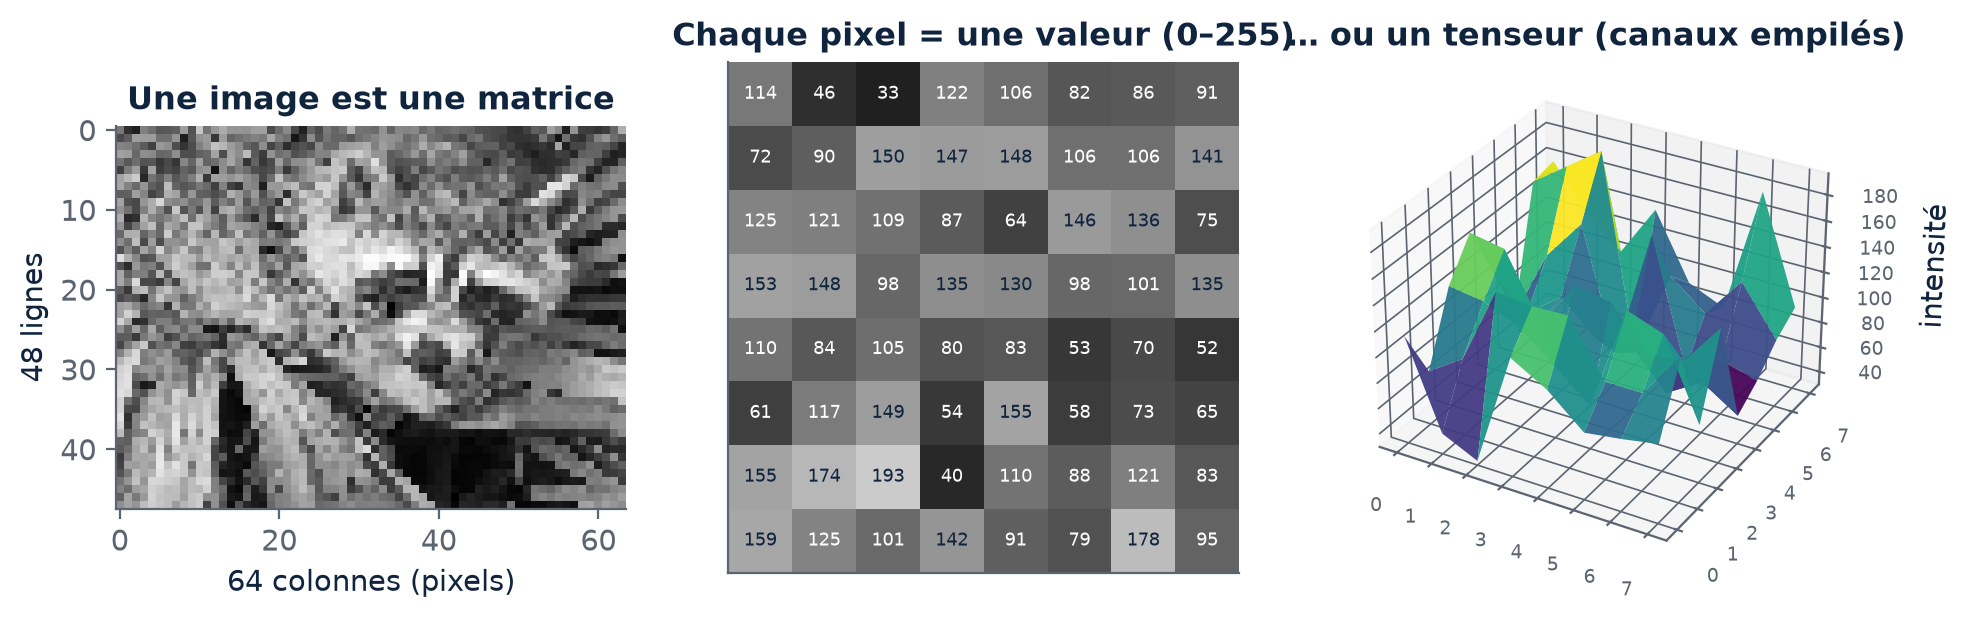
\includegraphics[width=\textwidth]{f02_matrice_tenseur.png}
\end{column}
\begin{column}{0.50\textwidth}
\begin{itemize}
  \item Une image en niveaux de gris est de \textbf{une seule matrice} :
  chaque élément est la luminosité d'un pixel (entier de 0 à 255).
  \item Une image \textbf{couleur} est un \textbf{tenseur} de trois matrices
  empilées : rouge, vert, bleu.
  \item Un pixel n'est donc pas un nombre isolé : c'est un nombre
  \textbf{à une position}.
\end{itemize}
\begin{kbox}[Vocabulaire]
\textbf{Tenseur} = tableau à $n$ dimensions. Une matrice est un tenseur d'ordre 2 ;
une image couleur, d'ordre 3.
\end{kbox}
\end{column}
\end{columns}
\end{frame}

\begin{frame}[fragile]{Le catalogue MNIST : 28 pixels par 28}
\begin{columns}[t]
\begin{column}{0.55\textwidth}
\begin{itemize}
  \item Le jeu de données de référence des débuts : 70\,000 chiffres manuscrits,
  28$\times$28 pixels, en niveaux de gris.
  \item Chaque image contient $28 \times 28 = 784$ valeurs.
  \item Un MLP exige un \textbf{vecteur} : il faut donc « aplatir » la matrice
  en concaténant les lignes.
  \item Opération \file{flatten} : la structure spatiale disparaît.
\end{itemize}
\begin{wbox}[Le premier piège]
Aplatir une image, c'est perdre l'information la plus précieuse : deux pixels
voisins sont liés, deux pixels opposés ne le sont pas.
\end{wbox}
\end{column}
\begin{column}{0.42\textwidth}
\begin{codebox}[Aplatir une image en Python]
\begin{lstlisting}
import numpy as np
img = np.zeros((28, 28))    # une image
v = img.flatten()           # 784 valeurs
print(v.shape)              # (784,)

# reconstruction : la structure
# doit etre stockee ailleurs
img2 = v.reshape(28, 28)
\end{lstlisting}
\end{codebox}
\end{column}
\end{columns}
\end{frame}

\begin{frame}{Les applications qui ont rendu les CNN incontournables}
\begin{columns}[t]
\begin{column}{0.31\textwidth}
\begin{ebox}[Classification d'images]
Attribuer une étiquette à une image entière : \emph{chat}, \emph{panneau STOP},
\emph{chiffre 4}. C'est la tâche fondatrice.
\end{ebox}
\begin{ebox}[Détection d'objets]
Localiser \emph{et} classer : une ou plusieurs boîtes englobantes par image.
\end{ebox}
\end{column}
\begin{column}{0.31\textwidth}
\begin{ebox}[Segmentation]
Attribuer une classe à \emph{chaque pixel} : sémantique, par instance, panoptique.
Indispensable en imagerie médicale et en conduite autonome.
\end{ebox}
\begin{ebox}[Séries temporelles]
Un signal 1D (ECG, trafic, météo) se traite avec les mêmes principes : la
convolution devient unidimensionnelle.
\end{ebox}
\end{column}
\begin{column}{0.31\textwidth}
\begin{ebox}[Reconnaissance faciale]
Empreintes, appariement, contrôle d'accès. Le CNN est le composant de base.
\end{ebox}
\begin{ebox}[Landmarking]
Poser automatiquement des points anatomiques sur des images : morphométrie,
analyse de forme, étude de populations.
\end{ebox}
\end{column}
\end{columns}
\end{frame}

\begin{frame}{Repères historiques}
\begin{center}
\begin{tabular}{@{}lll@{}}
\toprule
\textbf{Année} & \textbf{Étape} & \textbf{Idée retenue} \\
\midrule
1943 & Neurone formel (McCulloch--Pitts) & modèle mathématique du neurone \\
1958 & Perceptron (Rosenblatt) & apprentissage supervisé linéaire \\
1980 & Neocognitron (Fukushima) & localité et hiérarchie de motifs \\
1986 & Rétropropagation (Rumelhart \emph{et al.}) & entraîner des réseaux profonds \\
\textbf{1998} & \textbf{LeNet-5 (LeCun)} & la convolution \emph{apprise} : premier CNN opérationnel \\
2012 & AlexNet (Krizhevsky \emph{et al.}) & GPU + données massives, bascule de l'IA \\
2014 & VGG, GoogleNet & la profondeur devient un principe \\
2015 & ResNet (He \emph{et al.}) & connexions sautées, réseaux très profonds \\
2012--auj. & segmentation, détection, génération & les CNN partout \\
\bottomrule
\end{tabular}
\end{center}
\vspace{1mm}
\begin{kbox}[À retenir]
Fukushima pose l'idée en 1980, LeCun la rend \emph{apprenable} en 1998 ; le trio
\emph{données -- GPU -- profondeur} la transforme en révolution en 2012.
\end{kbox}
\end{frame}

\begin{frame}{Quiz d'entrée}
\begin{qbox}[Question 1]
Une image en couleur de $1\,000 \times 1\,000$ pixels : combien de nombres
contient-elle ?
\begin{itemize}
  \item[(a)] 1 million \quad (b) 3 millions \quad (c) 1 milliard
\end{itemize}
\end{qbox}
\begin{qbox}[Question 2]
Pourquoi un perceptron multicouche exige-t-il d'« aplatir » une image ?
\begin{itemize}
  \item[(a)] Pour aller plus vite \quad (b) Parce qu'il attend un \emph{vecteur} en entrée
  \quad (c) Parce que cela améliore la précision
\end{itemize}
\end{qbox}
\begin{qbox}[Question 3]
Deux motifs identiques placés à deux endroits différents de l'image :
un MLP les reconnaît-il de la même manière ?
\begin{itemize}
  \item[(a)] Oui, toujours \quad (b) Non, les connexions dépendent de la position
  \quad (c) Oui, si l'image est normalisée
\end{itemize}
\end{qbox}

% [fix] bloc deplace
\end{frame}
\begin{frame}{Quiz d'entrée (suite)}
\begin{solbox}[Réponses --- à ne regarder qu'après avoir répondu]
\textbf{1.} (b) : trois canaux, donc $3 \times 10^6$ valeurs. \quad
\textbf{2.} (b) : l'entrée d'un MLP est un vecteur, la structure spatiale est perdue. \quad
\textbf{3.} (b) : chaque connexion est liée à \emph{une} position ; rien n'est partagé.
\end{solbox}
\end{frame}
